\documentclass[12pt,crop=false,class=article,convert={density=300,outext=.compiled.png}]{standalone}
\usepackage{postmacs}
\usepackage{mathmacs}


\title{\Huge Movie Reviews and Gradient Descent 
}
\date{}
\author{Nithish Divakar}

\begin{document}
\maketitle


The problem is simple, $m$ movies, $n$ users and we have the data of rating of movies by users. Now in reality, each user might have rated a few movies while total number of users and movies are huge. We can consider the whole ratings data as a matrix $n\times m $ matrix $R$ where $R_{ij}$  is the rating of $i^{th}$ movie by $j^{th}$ user.


The problem is to have a system which can predict the rating a user would have given a movie. Now the modelling part is easy as a matrix factorisation problem. We can assume every user is represented by a embedding $u_i$  and similarly, every movie has a embedding $m_j$. We simply want 

$$M_{ij}  \sim \transpose{ u_i}m_j$$


If we simply model the learning problem as $$ \argmin_{U,M} \| \transpose{U}M - R \|_2$$ then we are implicitly assuming that all unavailable ratings are low (0). Since we have only a few ratings compared to all possible combinations of movies and users, this is not an assumption we can make. 

\section*{Good Modelling}

What we need to do instead is to simply model what the data is available us and nothing else.  Essentially, 

$$\argmin_{u_i,m_j}  \sum_{(u_i,m_j,r_{ij})\in D} \left(\transpose{u_i}m_j - r_{ij}\right)^2$$


\section*{Gradient Descent and Training}

The updates for U and M according to gradient descent are

$$u_i \gets u_i -  2\alpha (\transpose{u_i}m_j  - r_{ij})m_j$$

$$m_j \gets m_j - 2\alpha (\transpose{u_i}m_j  - r_{ij})u_i$$


Now to convert this to a batched gradient descent, we simply have to take a batch of ratings + indices and work on updating only the concerned indices of $U$ and $M$. But we have to handle the case where \textbf{user id or movie id is repeated in our batch}. The gradient have to be averaged in such case. The following code does it, but slowly. 

%{\centering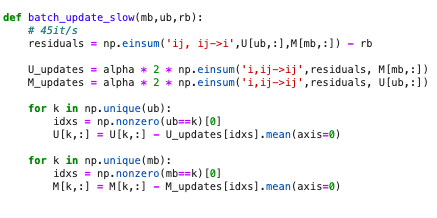
\includegraphics[width=0.99\textwidth]{../images/014_slow_batch_update.png}}

\begin{lstlisting}[language=Python]
def batch_update_slow(mb,ub,rb):
    # 45it/s
    residuals = np.einsum('ij, ij->i',U[ub,:],M[mb,:]) - rb

    U_updates = alpha * 2 * np.einsum('i,ij->ij',residuals, M[mb,:])
    M_updates = alpha * 2 * np.einsum('i,ij->ij',residuals, U[ub,:])
    
    for k in np.unique(ub):
        idxs = np.nonzero(ub==k)[0]
        U[k,:] = U[k,:] - U_updates[idxs].mean(axis=0)
    
    for k in np.unique(mb):
        idxs = np.nonzero(mb==k)[0]
        M[k,:] = M[k,:] - M_updates[idxs].mean(axis=0)
\end{lstlisting}

Vectorising the same code requires calculation of all gradients and then scaling it using frequency of each indices. The scaled gradients of each indices can them simply be added together to effectively get average gradient from each repeated indices.  The vectorised version is significantly faster.


\begin{lstlisting}[language=Python]

def batch_update(mb,ub,rb):
    # 800it/s
    
    # U <- U - 2a(U^TM-rb)M
    # M <- M - 2a(U^TM-rb)U
    
    residuals = np.einsum('ij, ij->i',U[ub,:],M[mb,:]) - rb

    # U[ub,:] = U[ub,:] - alpha * 2 * residue * M[mb,:]
    # M[mb,:] = M[mb,:] - alpha * 2 * residue * U[ub,:]

    ## Update U
    
    # get unique user_ids, reverse mappings, and counts of each user_ids
    idxs,ixds, cnt = np.unique(ub,return_inverse=True, return_counts=True)
    
    # get frequency of each indices
    frequency = (1.0/cnt)[ixds]
    
    # compute full gradient, then scale each gradient by frequency 
    
    # gradient            = np.einsum('ij,i->ij',M[mb,:],residuals)
    # scaled_gradient     = np.einsum('ij,i->ij',gradient,frequency)
    scaled_gradient     = np.einsum('ij,i,i->ij',M[mb,:],residuals,frequency)
    
    # Sum scaled gradient for unique user ids together
    
    F = lambda w: np.bincount(ixds,weights=w)
    aggregated_gradient = np.apply_along_axis(F,0, scaled_gradient)
    
    # update U with the gradients
    U[idxs,:] = U[idxs,:] - alpha * 2 * aggregated_gradient
    
    
    ## Update M (similar steps as U)
    idxs,ixds, cnt = np.unique(mb,return_inverse=True, return_counts=True)
    frequency = (1.0/cnt)[ixds]
    
    # gradient            = np.einsum('ij,i->ij',M[mb,:],residuals)
    # scaled_gradient     = np.einsum('ij,i->ij',gradient,frequency)
    scaled_gradient     = np.einsum('ij,i,i->ij',U[ub,:],residuals,frequency)
    
    F = lambda w: np.bincount(ixds,weights=w)
    aggregated_gradient = np.apply_along_axis(F,0, scaled_gradient)
    
    M[idxs,:] = M[idxs,:] - alpha * 2 * aggregated_gradient

\end{lstlisting}

\end{document}
